\documentclass{article}

% if you need to pass options to natbib, use, e.g.:
% \PassOptionsToPackage{numbers, compress}{natbib}
% before loading nips_2018

% ready for submission
%\usepackage{nips_2018}

% to compile a preprint version, e.g., for submission to arXiv, add
% add the [preprint] option:
\usepackage[preprint]{nips_2018}

% to compile a camera-ready version, add the [final] option, e.g.:
% \usepackage[final]{nips_2018}

% to avoid loading the natbib package, add option nonatbib:
% \usepackage[nonatbib]{nips_2018}
% For citations

\usepackage[utf8]{inputenc} % allow utf-8 input
\usepackage[T1]{fontenc}    % use 8-bit T1 fonts
\usepackage{hyperref}       % hyperlinks
\usepackage{url}            % simple URL typesetting
\usepackage{booktabs}       % professional-quality tables
\usepackage{amsfonts}       % blackboard math symbols
\usepackage{nicefrac}       % compact symbols for 1/2, etc.
\usepackage{microtype}      % microtypography
\usepackage{graphicx}

% For algorithms
\usepackage{algorithm}
\usepackage{algorithmic}
\usepackage{amsfonts}
\usepackage{amstext}
\usepackage{amssymb}
\usepackage{amsmath}

\usepackage{caption}

\title{Toward Dispelling Unhelpful Explainable Machine Learning (ML) Misconceptions}

% The \author macro works with any number of authors. There are two
% commands used to separate the names and addresses of multiple
% authors: \And and \AND.
%
% Using \And between authors leaves it to LaTeX to determine where to
% break the lines. Using \AND forces a line break at that point. So,
% if LaTeX puts 3 of 4 authors names on the first line, and the last
% on the second line, try using \AND instead of \And before the third
% author name.

% Authors in alphabetical order
\author{
  Patrick Hall\thanks{H2O.ai and George Washington University}\\
  Washington, DC\\
  \texttt{patrick.hall@h2o.ai}}

\begin{document}

\maketitle

\begin{abstract}

This short text presents arguments, proposals, and references to address recently uncovered misinformation and misconceptions about explainable machine learning. It also argues that post-hoc explanatory methods are one of several viable types of tools in a holistic, interpretable approach to machine learning.

\end{abstract}

\section{Introduction}

``Please stop doing explainable ML,'' extolled one of the brightest minds in machine learning with the title of a recent, well-reasoned, and admittedly controversial short talk. The same talk also included points such as, ``[Explainable ML] forces you to rely on two models instead of one,'' and argued that explainable machine learning can be a foil for companies and governments to conduct unsavory or negligent deeds with black-box models. \footnote{Statistics at a Crossroads, Webinar 2. URL: \url{https://zoom.us/recording/play/0y-iI9HamgyDzzP2k_jiTu6jB7JgVVXnjWZKDMbnyRTn3FsxTDZy6Wkrj3_ekx4J?startTime=1538497702000}} Perhaps even more noteworthy was the online response, which included musings such as, ``don’t forget hidden assumptions for explainable ML (e.g., locally linear behavior near predictions),'' and lamentations like, ``no one has explained to me what 'explainable' or 'interpretable' is.'' \footnote{Twitter thread: \url{https://twitter.com/tdietterich/status/1052680788389507073}} Strangely, neither the talk nor the follow-up discussions seemed to allow for combining white-box models and post-hoc explanatory techniques. This article aims to clear misconceptions and fill gaps in community knowledge exposed by these recent discussions. 

\begin{figure}[htb]
	\begin{center}
		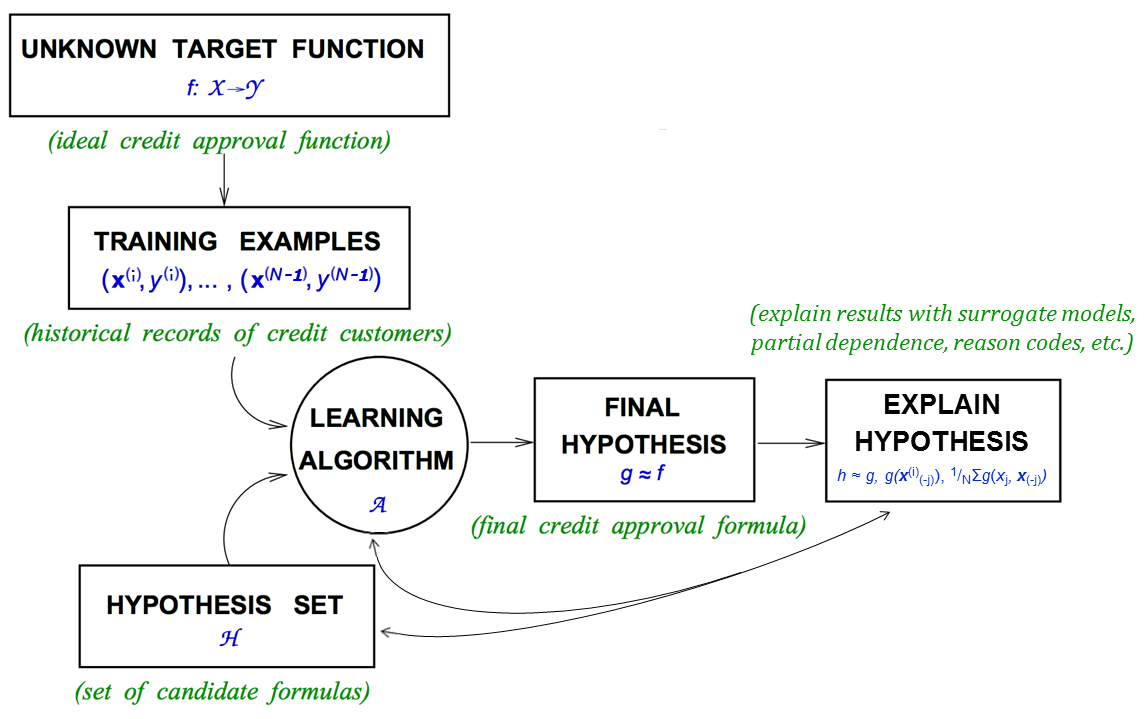
\includegraphics[scale=0.33]{img/figure_1.png}
		\label{fig:learning_problem}
		\captionsetup{labelformat=empty}
		\caption{\textbf{Figure:} An augmented learning problem diagram in which several post-hoc techniques create explanations for a credit scoring model. Adapted from \textit{Learning From Data} \cite{lfd}. <Suggestion(PC): We might want to add another 
		arrow from explanations going back to hypothesis(These explanations are helping us improve our assumptions and hypothesis>} 
	\end{center}
\end{figure}	

To avoid ambiguity and as illustrated in the figure below, here explainable ML means post-hoc techniques used to understand trained model behavior or predictions. Examples of common explainable ML techniques include:

\begin{itemize}
\item Local and global feature importance methods, in particular Shapley values \cite{keinan2004fair} \cite{kononenko2010efficient} \cite{shapley}.
\item Local and global model-agnostic surrogate models, such as surrogate decision trees and Local Interpretable Model-agnostic Explanations (LIME) \cite{dt_surrogate1}, \cite{dt_surrogate2}, \cite{lime-sup}, \cite{lime}. 
\item Local and global visualizations of model predictions such as partial dependence(1-way or 2-way interaction) and individual conditional expectation (ICE) plots \cite{esl}, \cite{ice_plots}.
\end{itemize}

By presenting definitions for key terms and at the same time addressing misconceptions, this text builds a case for a holistic approach to ML that includes white-box models along with explanatory, debugging, and fairness techniques. The article also implies that ignoring an entire set of methods because \textit{some subset} of the methods are approximate is akin to throwing the baby out with the bath water<Suggestion:PC should we rephrase this>). 

\paragraph{This text does not condone the use of black-box models with only cursory applications of low fidelity post-hoc explanatory methods -- that practice is likely lazy, irresponsible, and unethical, and also potentially dangerous.}

\section{Misconception: All the Key Terms in Explainable ML are Undefined}

While far from a complete vocabulary, at least two helpful definitions that apply to explainable ML have been put forward.

\begin{itemize}
\item \textbf{Interpretable}: ``The ability to explain or to present in understandable terms to a human'' -- in \textit{Towards a Rigorous Science of Interpretable Machine Learning} by Doshi-Velez and Kim (2017).
\item \textbf{A Good Explanation}: ``When you can no longer keep asking why'' -- in \textit{Explaining Explanations: An Approach to Evaluating Interpretability of Machine Learning} by Gilpin et al. (2018).
\end{itemize}

(From a literal reading of these two well-founded definitions, it would certainly appear that explanations contribute to some process being interpretable.)  

\section{Misconception: Explainable ML is Just Models of Models}

Models of models, or surrogate models, can be helpful explanatory tools, but they are usually approximate, low-fidelity explainers. Aside from the facts that 1.) a course, global summary of a complex model provided by a surrogate model can be helpful and 2.) much work in explainable ML has been directed toward improving the fidelity and usefulness of surrogate models \citep{dt_surrogate1}, \cite{dt_surrogate2}, \cite{lime-sup}, \cite{wf_xnn}, \textit{many explainable ML techniques have nothing to do with surrogate models!}   

One of the most exciting breakthroughs in explainable ML is tree shap, a model-specific (i.e. not a surrogate model), rigorously defined, accurate and consistent, global and local feature importance measure \cite{tree_shap}. There are many other explainable ML methods that operate on trained models directly such as partial dependence and ICE plots \cite{esl}, \cite{ice_plots}. Moreover, surrogate models and model-specific explanatory techniques can be combined, for instance by using partial dependence, ICE, and surrogate decision trees to investigate and confirm modeled interactions \cite{art_and_sci}. 

For a curated list of many different types of white-box modeling, model debugging, and model-specific, model-agnostic, and surrogate model explainable ML techniques, please see:
\begin{center}
\url{https://github.com/jphall663/awesome-machine-learning-interpretability}
\end{center}

\textbf{Misconception Corollary: Explainable ML is just LIME.} LIME, in it's most popular implementation, uses local linear surrogate models \cite{lime}. LIME is popular, important, and imperfect, but just one of many explainable ML tools. And again, LIME can sometimes be combined with model-specific methods to yield deeper insights. Consider that tree shap can provide locally accurate and consistent point estimates for local feature importance whereas LIME can provide approximate information about modeled local linear trends around the same point.   

\section{Misconception: Explainable ML Methods Simply Provide Cover For Government and Commercial Entities to Use Black-Box ML for Nefarious Purposes}

If used disingenuously, explainable ML methods probably do provide such cover, but explainable ML methods were designed to crack open those same nefarious black-boxes. See Angwin et al. (2016) for evidence that investigative analysis of commercial black-box models is possible \cite{angwin16}. Such investigations would likely only be improved by advances in explanatory, debugging, and fairness tools. \\

Additionally, many important computer-based technological advances present similar double-edged sword dilemmas, i.e. social media or strong encryption. Rarely does the ability of a tool to be misused for malicious purposes  disqualify it from being used as designed. Many explainable ML methods have already been implemented into open source software and are being used somewhat widely. The techniques need more public debate, scrutiny, and development, not dismissal and derision.

\section{Misconception: Explainable ML Methods and White-box Models are Somehow Mutually Exclusive}

Publications tend to focus on either white-box modeling techniques or on post-hoc explanations, but the two can be, and potentially should be, used together. Consider the seemingly useful cases of augmenting globally interpretable models with local post-hoc explanations, or the converse, combining global explanatory methods with locally interpretable models.

\begin{itemize}
\item \textbf{Proposed globally interpretable model + local explainability method example}: Using a single pruned decision tree with local Shapley feature importance to see accurate, numeric feature contributions for each model prediction in addition to the entire directed graph of the decision tree.
\item \textbf{Proposed locally interpretable model + global explainability method example}: Combining a locally interpretable rule-based classifier, that produces a rule list for each prediction, with partial dependence plots to aid in understanding the complex rule-based response function w.r.t. to each model input or pairwise combination of inputs.  
\end{itemize}

\textbf{Corollary Misconception: Explainable ML Methods and Fairness Methods are Somehow Mutually Exclusive}

Like white-box models, fairness methods are often presented in different articles than post-hoc explanatory methods. However, in banks, using partial dependence plots for model validation and disparate impact analysis for fair lending purposes for the same model is common place.

\section{Conclusion}

This short text is not an attack on any party. Much credible work has been done in several disciplines to make machine learning more interpretable, and thus better as a science. All of that work is likely less valuable in silos, and likely more valuable and practical when used in combination. Because work in white-box models, or in explanations, or in fairness, or in model debugging all typically requires both a deep understanding of machine learning and of other branches of science, say data visualization, optimization, or sociology, others might consider penning this type of short FAQ or summary article to elucidate details of their specialty to the broader community.    

%-------------------------------------------------------------------------------
%\section{References}
%-------------------------------------------------------------------------------

\bibliographystyle{plain}
\bibliography{xai_misconceptions}
\end{document}